\documentclass{gdl}

% CHANGE THESE
\def\groupid{BEK}
\def\projectid{AP-GCN}

\usepackage{subcaption}
\usepackage{float}

\DeclareMathOperator*{\argmin}{arg\,min}

\graphicspath{{figures/}}

\begin{document}

% CHANGE THIS
\title{AP-GCN Revisited: Replication and Alternative Approaches for Adaptive Propagation in Graph Neural Networks}

% CHANGE THIS
\author{%
Jonatan Bella, Tobias Erbacher, Jonas Knupp\\
\texttt{\{jonatan.bella, tobias.erbacher, jonas.knupp\}@usi.ch}
}

\begin{abstract}
\textcolor{red}{Concise and self-contained description of your project, motivation and main findings.}

% Delete the following part before submitting the report
\begin{center}
    \sf\large\color{red} GENERAL NOTES
\end{center}

\textcolor{red}{The report should be written as an article intended to present the findings of your work. Your aim should be to be clear and objective, substantiating your claims with references or empirical/theoretical evidence.
We are well aware of the fact that carrying out machine learning experiments might be difficult and that often the final performance might be disappointing. For this reason, you will not be evaluated solely on quantitative aspect of your work, but mainly on the quality of your analysis and report.
The length of the report should be between 4 and 8 pages (without considering references).}

\end{abstract}

\maketitle

\section{Introduction}

\textcolor{red}{Here you should clarify the context of your project and the problem you are dealing with. You should also make a brief summary of the main results and contributions (i.e., if you tried to replicate the results of an existing paper you should say if you were successful or not). The introduction should help the reader to follow along for the rest of the paper.}

This work is a replication study for the paper "Adaptive Propagation Graph Convolutional Network" by Spinelli et al. \cite{spinelli2021}. [Confirm that their results hold if they do]. Furthermore, we implemented and evaluated several different approaches for allowing an individual number of message passing steps per node. [Very briefly mention/explain these approaches and tell how results are in comparison with Spinelli]. 

Our code is available on GitHub\footnote{\url{https://github.com/TobiasErbacher/gdl}}.

\section{Related works}

\textcolor{red}{Give a brief summary of (some) existing methods that are related to you project. For instance, you can refer to~\citet{gilmer2017neural}, or simply~\cite{gilmer2017neural}, for introducing Message Passing Neural Networks. In this section it is important to provide readers references to the current state of the art and the foundations of the presented method. 
N.B.: When referencing a different approach, it is not necessary to provide a detailed description, only one/two brief sentences are enough. The interested readers can eventually read the referenced work. }


The main contribution of Spinelli et al. is the introduction of the Adaptive Propagation Graph Convolutional Network (AP-GCN) which enables each node to have an individual number of message passing steps.

Xu et al. \cite{xu2018} introduced Jumping Knowledge Networks which perform a fixed number of message passes for all nodes and then use per-node LSTM attention to calculate the weighted average over the hidden vectors of the message passing rounds.   

Liu et al. \cite{liu2019} presented GeniePath networks which not only use an attention mechanism to weight the contribution of neighboring nodes but also rely on an LSTM-like gating mechanism that controls the flow of information from one message passing step to the next. In principle, GeniePath networks can learn to stop propagating information individually for each node.

Lai et al. \cite{lai2020} presented Policy-GNN which consists of two modules: a meta-policy module that relies on Deep Q-Learning predicts the required number of message passing steps per node and a GNN module that uses the meta-policy to learn graph representations.

Banino et al. \cite{banino2021} proposed the PonderNet architecture, which dynamically adjusts its computational effort based on the complexity of the given problem. While the authors do not explicitly discuss PonderNet in the context of GNNs, the architecture itself is adaptable to various neural network designs.

Xiao et al. \cite{xiao2021} presented the Learning to Propagate (L2P) framework. They use a latent discrete variable for each node that represents its optimal number of message passing steps. These variables are learned using variational Expectation-Maximization.

Finkelshtein et al. \cite{finkelshtein2024} introduced Cooperative Graph Neural Networks (CO-GNNs) where nodes are in one of the states Standard, Listen, Broadcast, or Isolate. The message-passing behavior of each node is governed by its current state. Nodes in the Isolate state neither send nor receive messages, effectively halting their participation in the propagation process — a situation similar to the halting mechanism in AP-GCN.

\section{Methodology}

\textcolor{red}{
\textit{You can change the name of this section as you see fit.}\\
In this section you should give a description of the methodological aspects of your work, for instance how you modified an existing method to perform a particular task or to overcome a particular limitation. If your project is about reproducibility, here you should describe the method presented in the original paper.}

In this section we describe the AP-GCN by Spinelli et al. Furthermore, we introduce alternative architectures that allow each node to dynamically adjust its number of message passing steps.

\subsection{AP-GCN}
In traditional message-passing-based graph neural networks, the number of propagation steps is identical for all nodes in the graph. This uniformity implies that each node aggregates information from its neighbors through a fixed number of iterations, regardless of its individual characteristics or position within the graph structure. Spinelli et al. focus on the case where the message-passing is implemented by a Graph Convolution Network (GCN) \cite{kipf2017}. However, their approach is not limited to GCNs. The proposed adaptive propagation GCN (AP-GCN) allows each node in the graph to have an individual number of message passing iterations. 

A classifier is added to each node that predicts based on the hidden embedding after $k$ message-passing iterations whether the propagation should halt. The output of the classifer, $h^k_i$, is the probability the propagation should stop for node $i$ after iteration $k$.

$$ h^k_i = \sigma(\textbf{Q}\textbf{z}^k_i + q) $$

\noindent $\textbf{Q}$ and $q$ are trainable parameters and are shared between all nodes. There are two ways the propagation can stop. Firstly, the propagation stops if the number of propagations reaches a predefined maximum number of allowed steps $T$. Secondly, the propagation stops when the propagation budget has been used up. The budget is defined as $1-\epsilon$ where $\epsilon$ is a hyperparameter set a small value. When $k=K_i$ the budget for node $i$ has been reached after $k$ iterations and the propagation stops. 

$$ K_i = \argmin_{k' \in \{1, 2, ..., T\}} \sum_{k=1}^{k'} h_i^k \geq 1-\epsilon $$

\noindent Knowing when the propagation stops allows us to define a cumulative distribution for the halting probabilities. TODO: are we sure about this (Remainder)?

\[
    p_i^k = 
    \begin{cases}
    R_i = 1 - \sum_{k=1}^{K_i - 1} h_i^k & \text{if } k = K_i \text{ or } k = T \\
    \frac{h_i^k}{\sum_{k=1}^{K_i} h_i^k} & \text{otherwise}
    \end{cases}
\]

\noindent The output of the AP-GCN message-passing layer for node $i$ is $\hat{\bf{z}}_i$. TODO: Why do we do this

$$ \hat{\bf{z}}_i = \frac{1}{K_i} \sum_{k=1}^{K_i} p_i^k \bf{z}^k_i + (1-p^k_i) \bf{z}_i^{k-1} $$

\noindent The propagation cost $\mathcal{S}_i$ for node $i$ is given by the sum of $K_i$ and $R_i$. Adding $\mathcal{S}_i$ to the loss term incentivizes the model to choose a limited number of propagation steps for node $i$. The propagation penalty $\alpha$ controls the trade-off between accuracy and compute time. A larger $\alpha$ encourages the model to restrict the number of propagation steps per node, whereas a smaller $\alpha$ allows for deeper message passing, potentially improving accuracy at the cost of increased computation. Spinelli et al. decided to update the halting unit once every five steps. 

$$ \mathcal{\hat{L}} = \mathcal{L} + \alpha \sum_{i\in \mathcal{V}} \mathcal{S}_i $$


\subsection{RL-AP-GCN}
The inherent dynamics of Graph Neural Network propagation, particularly the phenomenon where node representations tend to homogenize and converge, which can derive in over-smoothing, can serve as a powerful implicit signal for an adaptive halting mechanism to find an optimal halting point without the need to a computational regularization. An RL agent, observing the node's evolving embedding, can learn to recognize when the representation changes minimally between propagation steps and halt, ideally, in the maximum expressiveness of that particular node. This stabilisation indicates diminishing returns from further message passing, suggesting sufficient relevant neighborhood information has been aggregated at certain point. Consequently, the policy network can learn, guided purely by the task reward (e.g., classification accuracy), to halt propagation when this representational convergence occurs. This approach does not need for explicit regularization terms or penalties based solely on the number of steps, grounding the halting decision more organically in the information saturation relevant to solving the task, rather than an external computational budget.

The current reinforcement learning implementation treats each node as an Actor Critic agent but policy and value networks are shared among all nodes. We first compute the initial node embeddings. Then, an iterative loop begins where, at each step, the shared policy network (Actor) evaluates the current embedding of active nodes to output a halting probability, while a shared value network (Critic) estimates the expected future reward (baseline) from that state. A halting action is sampled (incorporating exploration noise during training), and propagation continues for non-halted nodes. Upon halting (or reaching the maximum iterations), a reward is calculated based primarily on the final classification correctness, and the system learns by back propagating a combined loss: a supervised loss for the GNN's classification output, and an RL loss comprising a policy gradient term (using the advantage calculated as actual reward minus the Critic's baseline), a value function loss for the Critic, and an entropy bonus to encourage exploration.

There are several extensions that could enhance the implementation. The sparse, delayed reward signal could be augmented with denser, intermediate rewards reflecting confidence gains at each step. The RL state representation could be enriched beyond the current embedding to include neighboring node embeddings difference or a history of embeddings (using RNNs or attention), giving the policy more context. Employing more advanced RL algorithms like PPO for policy updates or GAE for advantage estimation could improve training stability and sample efficiency compared to the current REINFORCE-with-baseline approach. Finally, refining the training strategy, perhaps by alternating between supervised and RL optimization steps, could further stabilize learning and potentially improve final performance. In any case, the results seems promising considering that we did not undergo into a deep search for hyperparameters or even a careful reward design.
\subsection{Ponder-AP-GCN}
Deeply inspired by PonderNet paper, we implement its core ideas for the GNN adaptive halting problem. The central concept treats the node's decision at each step as a Bernoulli trial: halt with probability $\lambda_n$ or continue. This $\lambda_n$ represents the conditional probability of halting at step $n$, given the node hasn't halted previously. Running this sequence up to a maximum $N$ steps defines an unconditional halting distribution $p_n$  (the probability of halting exactly at step $n$), which generalizes the geometric distribution by allowing $\lambda_n$  to vary per step. With this theoretical background, the model is trained end-to-end by minimizing an expected loss function: the reconstruction loss (e.g., cross-entropy averaged over the outputs $y_n$  weighted by their corresponding halting probability $p_n$), plus a KL divergence term. This KL term acts as a regularizer, weighted by $\beta$, encouraging the learned distribution $p_n$  to stay close to a predefined prior geometric distribution $p_G$ . The advantage here is replacing unintuitive computational penalties with this KL term, where the prior's influence on the expected number of steps (which is $\frac{1}{\lambda_n}$  for a geometric prior with parameter  ) is easily interpretable. For instance, setting the prior parameter $\lambda_p = \frac{1}{N}$ encourages the model towards an average of $N$ steps.

Focusing directly into our implementation, the architecture starts with an initial MLP that processes node features, followed by recurrent GCN propagation steps - similar to AP-GCN authors. A key component is the shared linear halting unit computing logits at each step, which are passed through a sigmoid function to yield the conditional halting probabilities $lambda_n$. The unconditional halting distribution $p_n$  is then derived iteratively from these $\lambda_n$  values, ensuring the probabilities sum to one over the maximum N steps. The training loss combines the expected loss (weighted by $p_n$) and the KL divergence between the learned $p_n$ and the geometric prior $p_G$, scaled by $\beta$. Inference can be performed either by first computing the full distribution p and selecting the step via argmax or sampling, or potentially through the computationally efficient sequential Bernoulli sampling at each step as proposed in the original PonderNet paper.
\subsection{Gumbel-AP-GCN}
We modify the PonderNet implementation slightly. The core idea and implementation remains the same in the sense that we calculate the conditional and unconditional probabilities under the same logic. However, instead of calculating the expected loss, we employ the Gumbel-Softmax technique to draw a differentiable sample of a single halting step from the learned distribution $p_n$ during each training forward pass. Therefore, instead of computing the overall expected loss, we compute it from the output corresponding to the sampled step. This is combined with temperature annealing such that we start with a higher temperature for boosting exploration among steps to softer and more discrete selections once we are further down training. In addition, we set the kl divergence hyperparameter to 0, such that the halting policy is learned solely by optimizing the task performance at the sampled steps without explicit regularization. 

The architecture, as mentioned, is similar to PonderNet, with the difference that the loss samples a halt step using a Gumbel-Softmax with annealed temperature $\tau$. The cross entropy then is calculated using only the predictions corresponding to these sampled steps.  We could extend this further by simply applying the efficient sequential Bernoulli sampling to reduce even more the computational load with respect to the previous approaches, in addition, of enriching the state representation for the halting unit. 

\subsection{Co-AP-GCN}

\section{Implementation}

\textcolor{red}{
This section should be structured as follows (from the Reproducibility challenge template):
---
Briefly describe what you did and which resources did you use. E.g. Did you use author's code, did you re-implement parts of the pipeline, how much time did it take to produce the results, what hardware you were using and how long it took to train/evaluate. }

We independently implemented AP-GCN and compared our implementation with the reference code provided by Spinelli et al., available on their GitHub repository\footnote{\url{https://github.com/spindro/AP-GCN}}. We found that in cases where nodes reach the maximum propagation limit $T$ and are eligible to propagate further, the implementation by Spinelli et al. incorrectly reports one additional step, resulting in an off-by-one error. Importantly, the implementation does not actually perform an extra propagation step—it only misreports the number of steps taken.

For the loading of the \texttt{Citeseer}, \texttt{Cora-ML}, \texttt{PubMed}, \texttt{MS-Academic}, \texttt{A. Computer}, and \texttt{A. Photo} datasets we used the code provided by Spinelli et al.

We asked Prof. Spinelli, among other questions, why they placed the feature mapping layer that projects to the number of classes before the message passing layer. However, we did not receive a response to our email.

\subsection{Datasets}
\textcolor{red}{Describe the datasets you used and how you obtained them. }

We downloaded the \texttt{Citeseer} \cite{sen2008}, \texttt{Cora-ML} \cite{mccallum2000}, \texttt{PubMed} \cite{namata2012}, \texttt{MS-Academic} \cite{shchur2018}, \texttt{A. Computer}, and \texttt{A. Photo} datasets from the GitHub repository of Spinelli et al. along with the code to load them. The \texttt{A. Computer} and \texttt{A. Photo} datasets are portions of the Amazon co-purchase graph originally presented in \cite{mcauley2015}. In the \texttt{Microsoft Academic} dataset, the edges represent co-authorship while in the \texttt{Citeseer}, \texttt{Cora-ML}, and \texttt{PubMed} datasets, the edges represent citations. All these datasets consists of a single graph and are node classification problems. Only the largest connected component in each dataset is used. The features are bag of words representations of the papers' abstracts. 

\subsection{Hyperparameters}
\textcolor{red}{Describe how you set the hyperparameters and what was the source for their value (e.g. paper, code or your guess). }

For the experiments with AP-GCN we used the hyperparameters described by Spinelli et al. They are described in appendix \ref{lab:hyper-ap-gcn}.

\subsection{Experimental setup}
\textcolor{red}{Explain how you ran your experiments, e.g. the CPU/GPU resources and provide the link to your code and notebooks.}

We follow the experimental setup of Spinelli et al., splitting each dataset into a training, a validation, and a test set. Spinelli et al. follow the experimental setup of \cite{}. The validation set is used to detect early stopping, while the test set serves to evaluate the final model performance. The union of the training and validation is considered to be the "visible" or "development" set. For the \texttt{MS-Academic} dataset, the development set consists of 5,000 samples, whereas for all other datasets it contains 1,500 samples. This larger size is chosen for \texttt{MS-Academic} because a smaller development set of 1,500 samples would likely result in fewer than 20 samples per class. For each dataset, we use 20 random seeds, and for each seed, the model is trained five times with different weight initializations, resulting in 100 trained models per dataset for a fixed set of hyperparameters.

While Spinelli et al. provided the seeds for the train/validation/test split, there is still randomness because of the model initializations. Since Spinelli et al. did not provide a seed to account for this, we selected the seed $11$ to make the model initializations reproducible. 

We report the average accuracy when using a training set of 20 nodes per class, with uncertainties showing the 95\% confidence level calculated by bootstrapping. The uncertainty is defined as the larger absolute difference between the mean and the 2.5th or 97.5th percentile of the bootstrap distribution. This follows the code in the Jupyter notebook provided by Spinelli et al. In each run we also save when each node in the test set halts.

\subsection{Computational requirements}
\textcolor{red}{Provide information on computational requirements for each of your experiments. For example, the number of CPU/GPU hours and memory requirements. You'll need to think about this ahead of time, and write your code in a way that captures this information so you can later add it to this section. }

The experiments were conducted on a MacBook Pro with Apple M2 Pro Chip and 16 GB of memory. We used the \texttt{mps} backend of PyTorch.


\section{Results}

\textcolor{red}{In this section you should report the results of your work (e.g., the outcome of an empirical analysis). You should be objective and support your statements with empirical evidence.}

\begin{table*}[h]
    \small\sf\centering
    \caption{Average test set accuracies with 95\% confidence intervals, computed from 100 runs per model using 20 random seeds and 5 different initial weight settings per seed.}
    \begin{tabular}{l c c c c c c}
        \toprule
        Model & Citeseer & Cora-ML & PubMed & MS-Academic & A.Computer & A.Photo\\
        \midrule
        \texttt{RL-AP-GCN} &$74.65 \pm 0.29$&$81.60 \pm 1.38$&$77.16 \pm 0.42$&$88.32 \pm 0.41$&$79.94 \pm 0.52$&$88.89 \pm 0.43$ \\
        \texttt{Ponder-AP-GCN} &$74.80 \pm 0.31$&$82.14 \pm 0.31$&$76.37 \pm 0.41$&$91.29 \pm 0.12$&$83.41 \pm 0.25$&$91.27 \pm 0.23$ \\
        \texttt{Gumbel-AP-GCN} &$70.09 \pm 1.25$&$70.92 \pm 2.34$&$76.83 \pm 0.49$&$87.56 \pm 0.45$&$79.13 \pm 0.58$&$89.21 \pm 0.44$ \\
        \texttt{Co-AP-GCN}  \\
        \texttt{AP-GCN replication} &$75.88 \pm 0.27$&$83.69 \pm 0.33$&$78.98 \pm 0.40$&$91.66 \pm 0.14$&$83.26 \pm 0.34$&$90.68 \pm 0.32$\\
        \midrule
        \texttt{AP-GCN} & $76.12 \pm 0.24$ & $85.71 \pm 0.22$ & $79.80 \pm 0.34$ & $92.62 \pm 0.07$ & $85.18 \pm 0.23$ & $92.05 \pm 0.22$\\
        \bottomrule
    \end{tabular}
    \label{tab:table}
\end{table*}

Use figures, plots and tables (like \autoref{tab:table}) to present your results in a nice and readable way.

We report the results of our experiments with the AP-GCN, Graph PonderNet, RL, and CoGNN architectures. For each model architecture we report the distribution of the halting steps, i.e., the steps at which each node halts. Since we have data from 100 runs per model architecture, we first average the halting steps for each node over the 100 runs and then plot the distribution obtained using kernel density estimation (KDE) over these averaged halting steps per node. Note that because of the averaging and the KDE there can be probability mass at non-integer values even though in reality all the models can only halt after an integer number of steps. This approach follows the methodology used by Spinelli et al.


\subsection{AP-GCN}

\subsection{RL-AP-GCN}

\subsection{Ponder-AP-GCN}

\subsection{Gumbel-AP-GCN}

\subsection{Co-AP-GCN}

\begin{figure*}[p]
    \centering
    \begin{minipage}[t]{0.48\textwidth}
        \centering
        \begin{subfigure}[b]{0.7\textwidth}
            \centering
            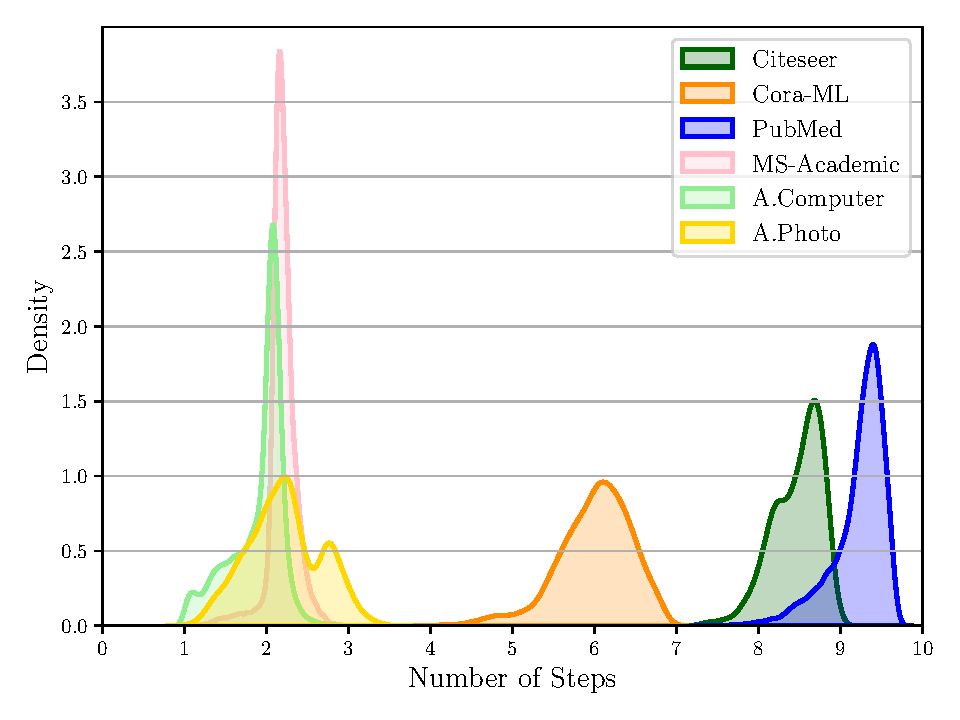
\includegraphics[width=\textwidth]{Spinelli_steps_distribution.pdf}
            \captionsetup{justification=centerlast}
            \caption{AP-GCN Replication}
            \label{fig:step_dist_AP_GCN}
        \end{subfigure}
        
        \begin{subfigure}[b]{0.7\textwidth}
            \centering
            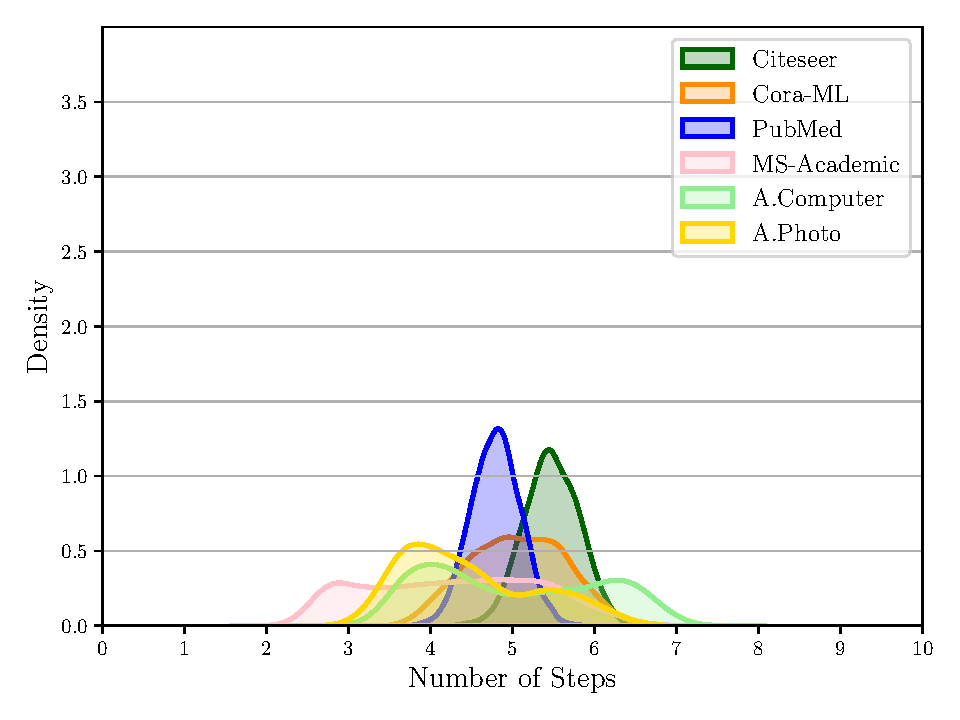
\includegraphics[width=\textwidth]{RL-AP-GCN_steps_distribution.pdf}
            \captionsetup{justification=centerlast}
            \caption{RL-AP-GCN}
            \label{fig:step_dist_RL_AP_GCN}
        \end{subfigure}
        
        \begin{subfigure}[b]{0.7\textwidth}
            \centering
            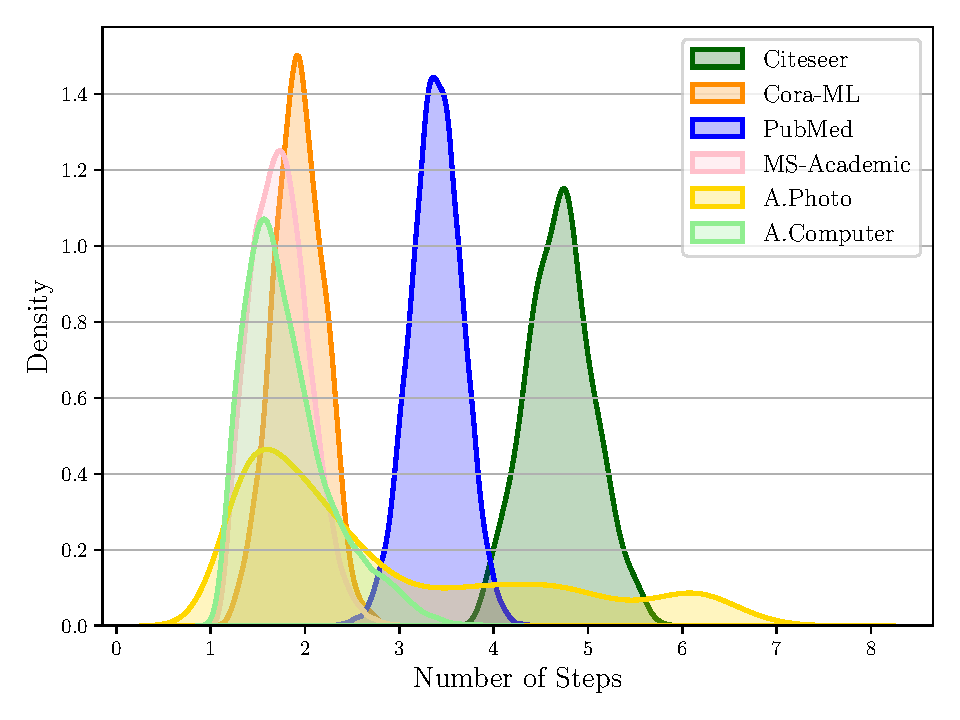
\includegraphics[width=\textwidth]{Ponder-AP-GCN_steps_distribution.pdf}
            \captionsetup{justification=centerlast}
            \caption{Ponder-AP-GCN}
            \label{fig:step_dist_Ponder_AP_GCN}
        \end{subfigure}
        
        \begin{subfigure}[b]{0.7\textwidth}
            \centering
            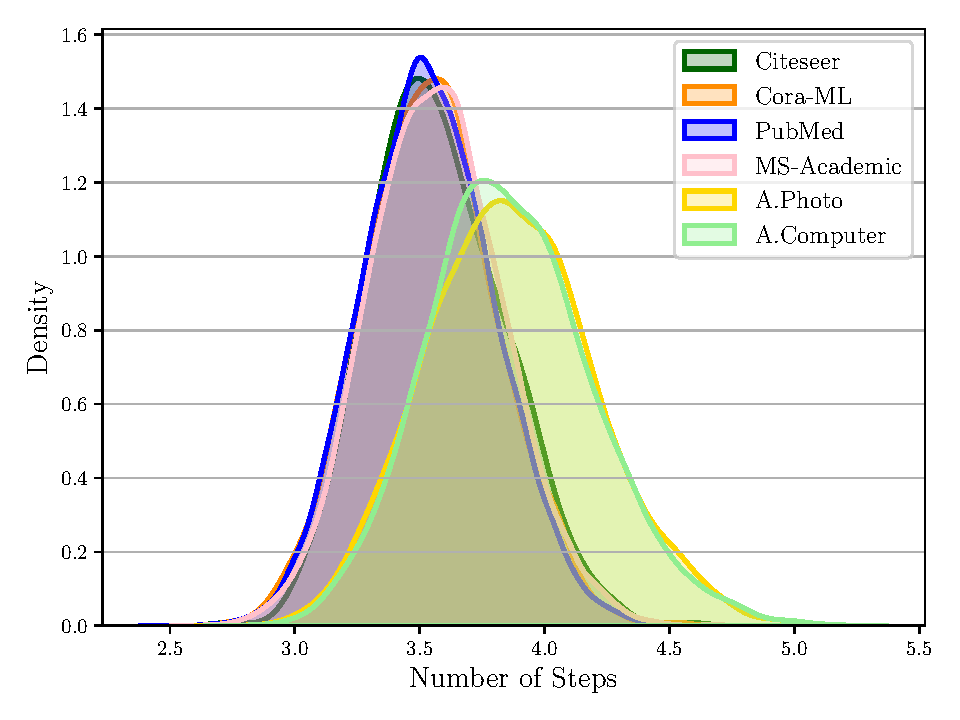
\includegraphics[width=\textwidth]{Gumbel-AP-GCN_steps_distribution.pdf}
            \captionsetup{justification=centerlast}
            \caption{Gumbel-AP-GCN}
            \label{fig:step_dist_Gumbel_AP_GCN}
        \end{subfigure}
        
        \begin{subfigure}[b]{0.7\textwidth}
            \centering
            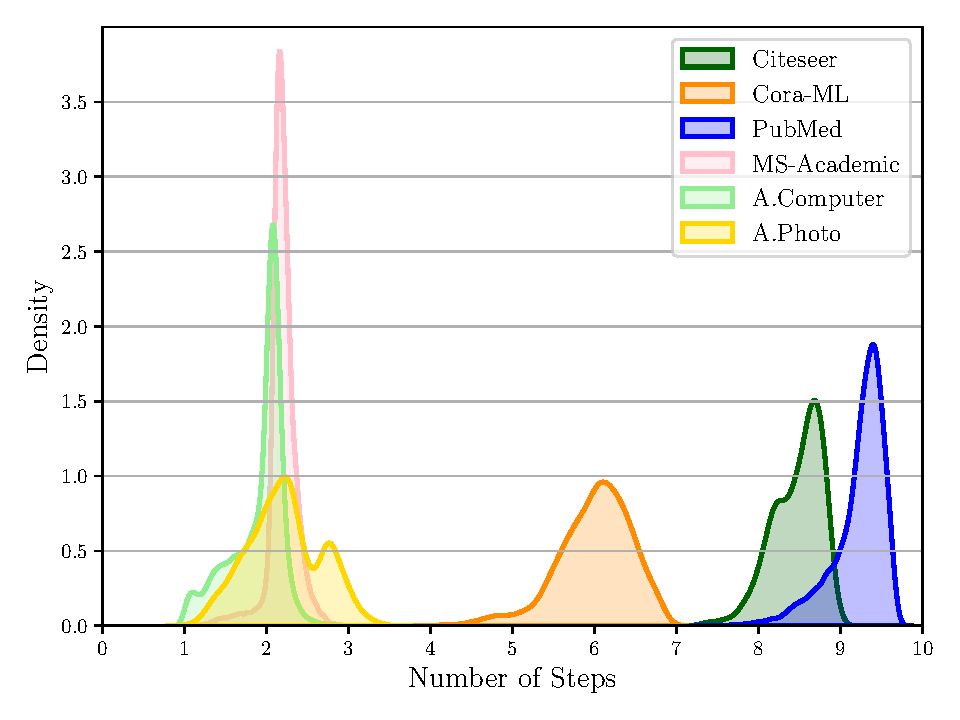
\includegraphics[width=\textwidth]{Spinelli_steps_distribution.pdf}
            \captionsetup{justification=centerlast}
            \caption{Co-AP-GCN}
            \label{fig:step_dist_Co_AP_GCN}
        \end{subfigure}
        
        \captionsetup{justification=centerlast}
        \caption{Average density distribution of the halting steps for the five different model architectures for each dataset.}
        \label{fig:main}
    \end{minipage}%
    \hfill
    \begin{minipage}[t]{0.48\textwidth}
        \centering
        \begin{subfigure}[b]{0.7\textwidth}
            \centering
            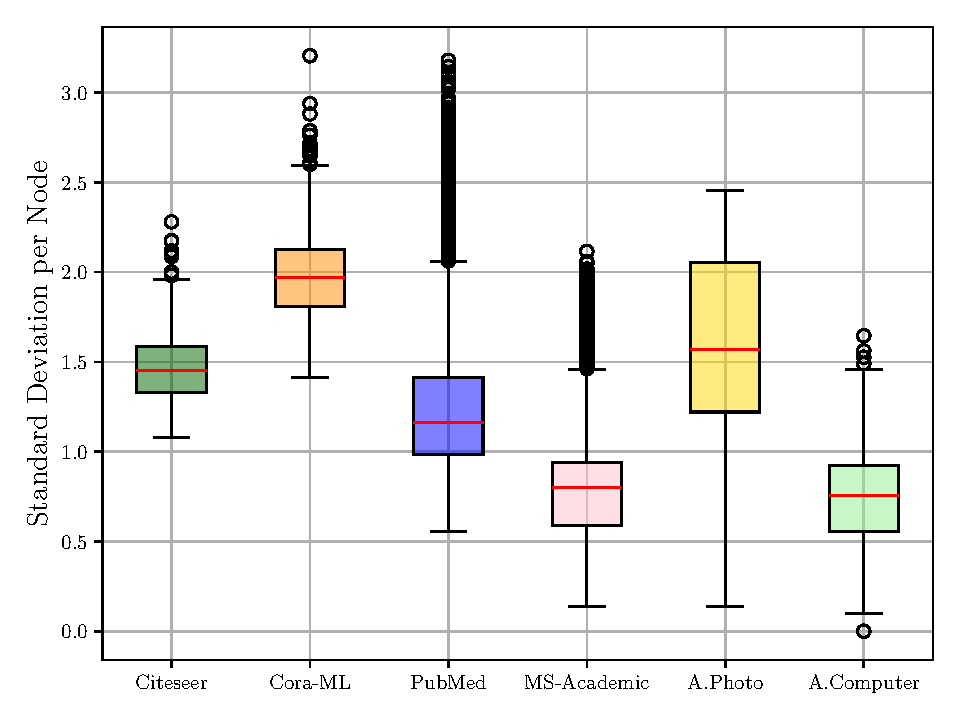
\includegraphics[width=\textwidth]{Spinelli_std_steps_per_node_boxplot.pdf}
            \captionsetup{justification=centerlast}
            \caption{AP-GCN Replication}
            \label{fig:step_std_AP_GCN}
        \end{subfigure}
        
        \begin{subfigure}[b]{0.7\textwidth}
            \centering
            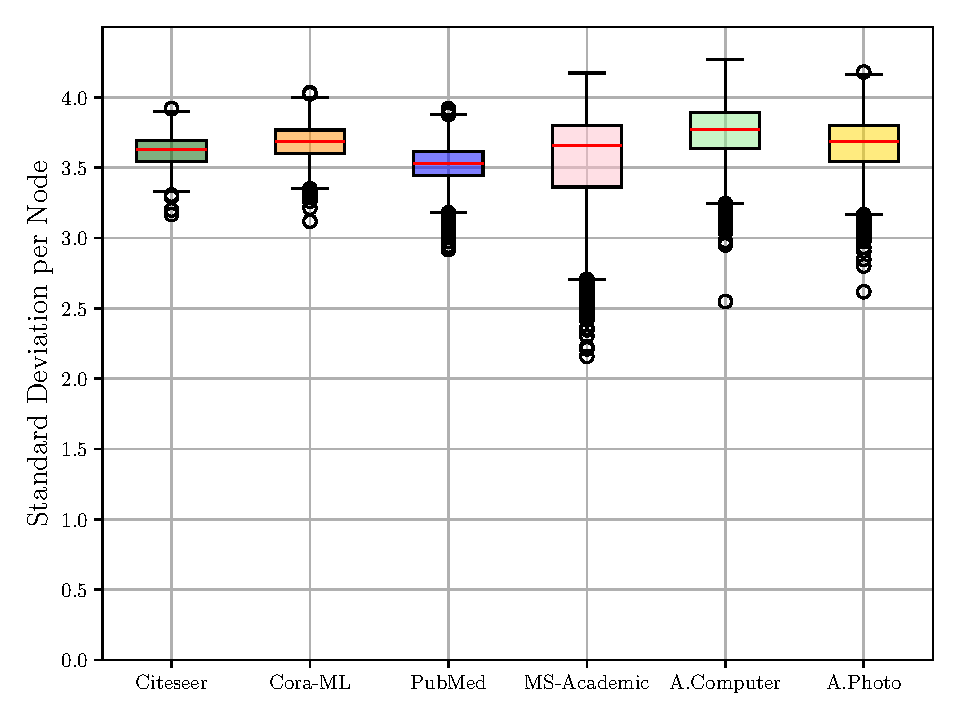
\includegraphics[width=\textwidth]{RL-AP-GCN_std_steps_per_node_boxplot.pdf}
            \captionsetup{justification=centerlast}
            \caption{RL-AP-GCN}
            \label{fig:step_std_RL_AP_GCN}
        \end{subfigure}
        
        \begin{subfigure}[b]{0.7\textwidth}
            \centering
            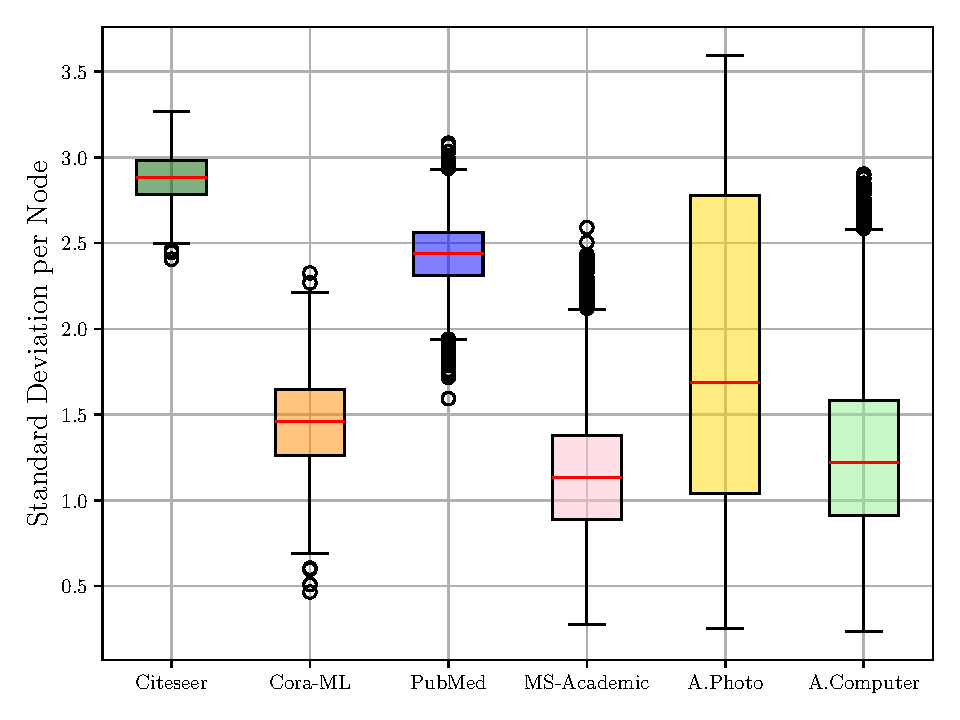
\includegraphics[width=\textwidth]{Ponder-AP-GCN_std_steps_per_node_boxplot.pdf}
            \captionsetup{justification=centerlast}
            \caption{Ponder-AP-GCN}
            \label{fig:step_std_Ponder_AP_GCN}
        \end{subfigure}
        
        \begin{subfigure}[b]{0.7\textwidth}
            \centering
            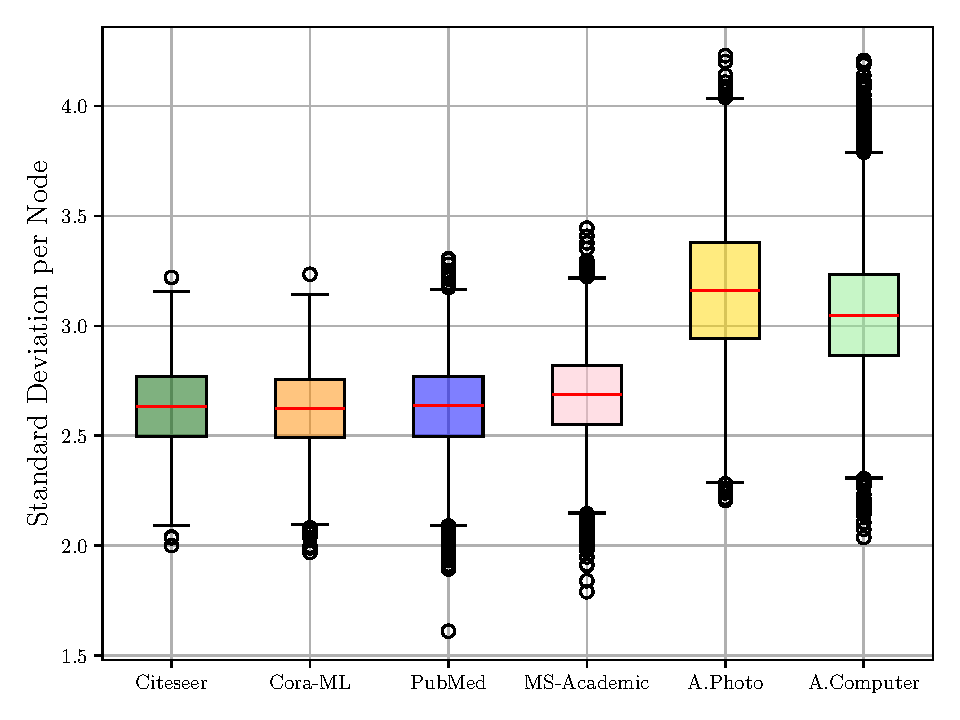
\includegraphics[width=\textwidth]{Gumbel-AP-GCN_std_steps_per_node_boxplot.pdf}
            \captionsetup{justification=centerlast}
            \caption{Gumbel-AP-GCN}
            \label{fig:step_std_Gumbel_AP_GCN}
        \end{subfigure}
        
        \begin{subfigure}[b]{0.7\textwidth}
            \centering
            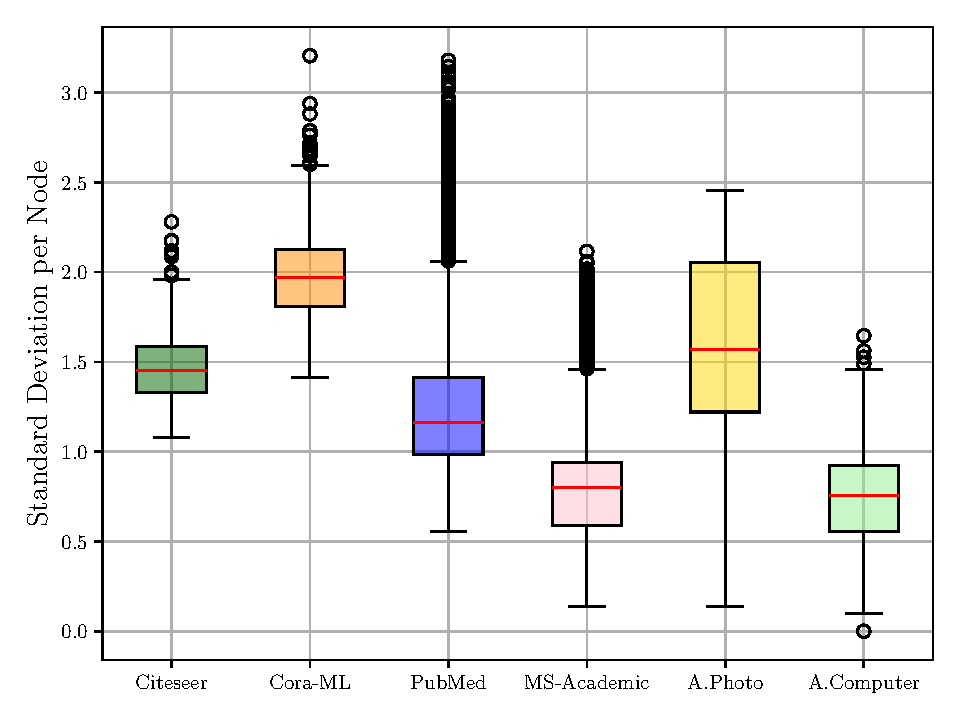
\includegraphics[width=\textwidth]{Spinelli_std_steps_per_node_boxplot.pdf}
            \captionsetup{justification=centerlast}
            \caption{Co-AP-GCN}
            \label{fig:step_std_Co_AP_GCN}
        \end{subfigure}
        
        \captionsetup{justification=centerlast}
        \caption{Standard deviations per node over the 100 experiments for each dataset.}
        \label{fig:steps_dist_steps_std}
    \end{minipage}
\end{figure*}


\section{Discussion and conclusion}

\textcolor{red}{Here you can express your judgments and draw your conclusions based on the  evidences produced on the previous sections.
Try to summarize the achievements of your project and its limits, suggesting (when appropriate) possible extensions and future works.}

\clearpage
% Bibliography
\bibliography{bibliography}
\bibliographystyle{unsrtnat}
\clearpage

\appendix

\section{Hyperparameters}

\subsection{AP-GCN}
\label{lab:hyper-ap-gcn}
We use 2 feature transformation layers, a dropout rate of 0.5, 64 hidden units, and the Adam optimizer with learning rate 0.01. The maximum number of steps $T$ was set to 10. We applied $L2$ regularization with coefficient 0.008 on the parameters of the first layer. For the \texttt{A. Photo} and \texttt{A. Computer} no regularization was used.


\end{document}
